\documentclass[a4paper,12pt]{article}
%\documentclass[fleqn]{article}

% ---パッケージ---
\usepackage{amsmath,amssymb}    %数式用
\usepackage{tcolorbox}   %囲み枠用(tcolorboxに変更)
\usepackage{geometry}   %余白調節
\usepackage{tikz}  % ← 図を描くためのTikZパッケージ
\geometry{margin=25mm}  %余白を少し狭く
\usetikzlibrary{decorations.pathmorphing,patterns,positioning,arrows.meta} % バネ・壁の模様
\tikzset{
  block/.style = {draw, rectangle, minimum height=2em, minimum width=3em},
  sum/.style = {draw, circle, inner sep=0pt, minimum size=5mm},
  input/.style = {coordinate},
  output/.style = {coordinate}
}
\usetikzlibrary{calc}
\usepackage{pgfplots}  % ← 追加(グラフ用)
\pgfplotsset{compat=newest} % ← 推奨設定

% --- 日本語用パッケージ ---
\usepackage{luatexja}         % 日本語表示に必要
\usepackage{luatexja-fontspec} % フォント指定用

% --- フォント指定(Overleaf標準フォント)---
\setmainjfont{IPAexMincho}  % 明朝体
%\setmainjfont{IPAexGothic}  % ゴシック体にしたい場合

% --- tcolorbox の設定 ---
\tcbset{
    colframe=black,
    colback=white,         % 本文の背景(白)
    boxrule=0.8pt,
    arc=3pt,
    outer arc=3pt,
    boxsep=4pt,
    coltitle=black,
    colbacktitle=gray!20,  % タイトルの背景(グレー)
    fonttitle=\normalsize
}

\begin{document}

\noindent
\text{制御工学Ⅰ 演習③ 解答}

\vspace{10mm}


% ---------------[1]--------------- 済
\noindent
1. 下図に示すシステムにおいて、システム全体の伝達関数を求めよ。\\
\begin{minipage}[t]{0.45\linewidth}
    (1)\\
    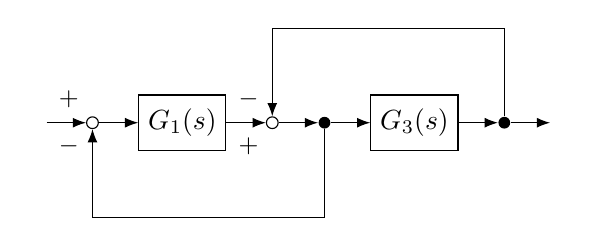
\begin{tikzpicture}[auto, node distance=0.3cm and 0.5cm, >=Latex]

        % --- 横並びのノード配置 ---
        \node at (0,0) (input) {};
        \node[circle, draw, inner sep=1.5pt, right=of input] (sum1) {};         % 合流1
        \node[block, right=of sum1] (G1) {$G_1(s)$};
        \node[circle, draw, inner sep=1.5pt, right=of G1] (sum2) {};            % 合流2
        \node[circle, fill=black, inner sep=1.5pt, right=of sum2] (branch1) {}; % 分岐1
        \node[block, right=of branch1] (G3) {$G_3(s)$};
        \node[circle, fill=black, inner sep=1.5pt, right=of G3] (branch2) {};   % 分岐2
        \node[right=of branch2] (output) {};

        % --- フィードバック座標ノード(図形なし) ---
    \coordinate (fb1) at ($(branch1)+(0,-1.2)$);
    \coordinate (fb2) at ($(branch2)+(0,1.2)$);

        % === 主系列 ===
        \draw[->] (input) -- (sum1);
        \draw[->] (sum1) -- (G1);
        \draw[->] (G1) -- (sum2);
        \draw[->] (sum2) -- (branch1);
        \draw[->] (branch1) -- (G3);
        \draw[->] (G3) -- (branch2);
        \draw[->] (branch2) -- (output);

        % === フィードバック経路 ===
        \draw[->] (branch1) |- (fb1.center) -| (sum1);
        \draw[->] (branch2) |- (fb2.center) -| (sum2);

        % --- 加算記号配置 ---
        \node at ($(sum1)+(-0.3,0.3)$) {\small $+$};
        \node at ($(sum1)+(-0.3,-0.3)$) {\small $-$};
        \node at ($(sum2)+(-0.3,0.3)$) {\small $-$};
        \node at ($(sum2)+(-0.3,-0.3)$) {\small $+$};


    \end{tikzpicture}\\

    (3)\\
    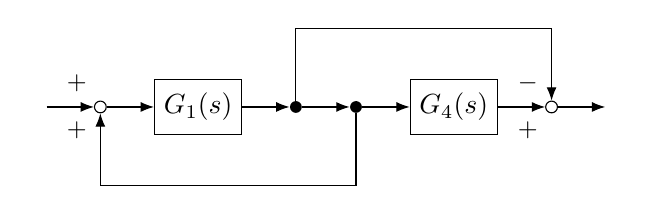
\begin{tikzpicture}[auto, node distance=0.4cm and 0.6cm, >=Latex]

            % --- 横並びノード ---
            \node at (0,0) (input) {};
            \node[circle, draw, inner sep=1.5pt, right=of input] (sum1) {};            % 合流1
            \node[block, right=of sum1] (G1) {$G_1(s)$};
            \node[circle, fill=black, inner sep=1.5pt, right=of G1] (branch1) {};      % 分岐1
            \node[circle, fill=black, inner sep=1.5pt, right=of branch1] (branch2) {}; % 分岐2
            \node[block, right=of branch2] (G4) {$G_4(s)$};
            \node[circle, draw, inner sep=1.5pt, right=of G4] (sum2) {};               % 合流2
            \node[right=of sum2] (output) {};
            
            % --- フィードバック座標 ---
            \coordinate (fb_down) at ($(branch2)+(0,-1.0)$);
            \coordinate (fb_up) at ($(branch1)+(0,1.0)$);
            
            % === 主系列 ===
            \draw[->] (input) -- (sum1);
            \draw[->] (sum1) -- (G1);
            \draw[->] (G1) -- (branch1);
            \draw[->] (branch1) -- (branch2);
            \draw[->] (branch2) -- (G4);
            \draw[->] (G4) -- (sum2);
            \draw[->] (sum2) -- (output);
            
            % === フィードバック経路 ===
            \draw[->] (branch2) |- (fb_down) -| (sum1);
            \draw[->] (branch1) |- (fb_up) -| (sum2);
            
            % --- 加算記号配置 ---
            \node at ($(sum1)+(-0.3,0.3)$) {\small $+$};
            \node at ($(sum1)+(-0.3,-0.3)$) {\small $+$};
            \node at ($(sum2)+(-0.3,0.3)$) {\small $-$};
            \node at ($(sum2)+(-0.3,-0.3)$) {\small $+$};
            
    \end{tikzpicture}
\end{minipage}
\hfill
\begin{minipage}[t]{0.45\linewidth}
    (2)\\
    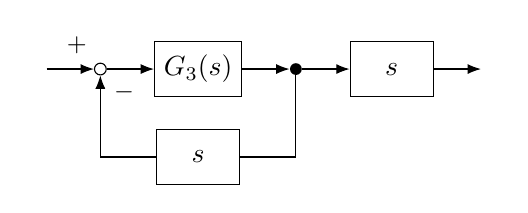
\begin{tikzpicture}[auto, node distance=0.4cm and 0.6cm, >=Latex]

        % --- 横並びの主系列ノード ---
        \node at (0,0) (input) {};
        \node[circle, draw, inner sep=1.5pt, right=of input] (sum) {};
        \node[block, right=of sum] (G3) {$G_3(s)$};
        \node[circle, fill=black, inner sep=1.5pt, right=of G3] (branch) {};
        \node[block, right=of branch] (s1) {$s$};
        \node[right=of s1] (output) {};
        
        % --- 下の s ノード ---
        \node[block, below=of G3] (s2) {$s$};
        
        % === 主系列 ===
        \draw[->] (input) -- (sum);
        \draw[->] (sum) -- (G3);
        \draw[->] (G3) -- (branch);
        \draw[->] (branch) -- (s1);
        \draw[->] (s1) -- (output);
        
        % === フィードバック経路(下) ===
        \draw[->] (branch) |- (s2) -| (sum);
        
        % --- 加算記号配置 ---
        \node at ($(sum)+(-0.3,0.3)$) {\small $+$};
        \node at ($(sum)+(0.3,-0.3)$) {\small $-$};
        
    \end{tikzpicture}\\

    (4)\\
    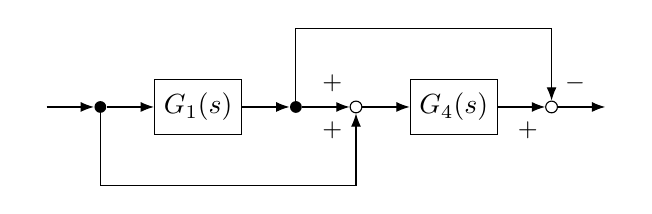
\begin{tikzpicture}[auto, node distance=0.4cm and 0.6cm, >=Latex]

        % --- 横並びノード(sum1 と branch2 の位置を交換) ---
        \node at (0,0) (input) {};
        \node[circle, fill=black, inner sep=1.5pt, right=of input] (branch2) {};     % ← 分岐2
        \node[block, right=of branch2] (G1) {$G_1(s)$};
        \node[circle, fill=black, inner sep=1.5pt, right=of G1] (branch1) {};        % 分岐1
        \node[circle, draw, inner sep=1.5pt, right=of branch1] (sum1) {};            % ← 合流1
        \node[block, right=of sum1] (G4) {$G_4(s)$};
        \node[circle, draw, inner sep=1.5pt, right=of G4] (sum2) {};                 % 合流2
        \node[right=of sum2] (output) {};
        
        % --- フィードバック座標 ---
        \coordinate (fb_down) at ($(branch2)+(0,-1.0)$);
        \coordinate (fb_up) at ($(branch1)+(0,1.0)$);
        
        % === 主系列 ===
        \draw[->] (input) -- (branch2);
        \draw[->] (branch2) -- (G1);
        \draw[->] (G1) -- (branch1);
        \draw[->] (branch1) -- (sum1);
        \draw[->] (sum1) -- (G4);
        \draw[->] (G4) -- (sum2);
        \draw[->] (sum2) -- (output);
        
        % === フィードバック経路 ===
        \draw[->] (branch2) |- (fb_down) -| (sum1);
        \draw[->] (branch1) |- (fb_up) -| (sum2);
        
        % --- 加算記号配置 ---
        \node at ($(sum1)+(-0.3,0.3)$) {\small $+$};
        \node at ($(sum1)+(-0.3,-0.3)$) {\small $+$};
        \node at ($(sum2)+(-0.3,-0.3)$) {\small $+$};
        \node at ($(sum2)+(0.3,0.3)$) {\small $-$};
        
    \end{tikzpicture}
\end{minipage}\\


\begin{tcolorbox}[title={1. (1)
    \vspace{-6mm}
    \begin{center}
        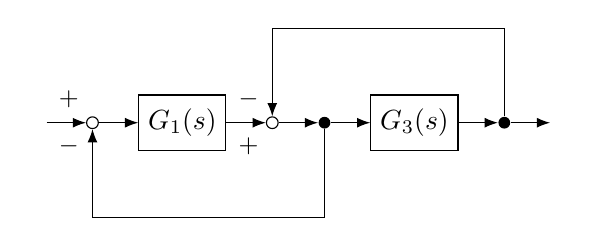
\begin{tikzpicture}[auto, node distance=0.3cm and 0.5cm, >=Latex]

        % --- 横並びのノード配置 ---
        \node at (0,0) (input) {};
        \node[circle, draw, inner sep=1.5pt, right=of input] (sum1) {};         % 合流1
        \node[block, right=of sum1] (G1) {$G_1(s)$};
        \node[circle, draw, inner sep=1.5pt, right=of G1] (sum2) {};            % 合流2
        \node[circle, fill=black, inner sep=1.5pt, right=of sum2] (branch1) {}; % 分岐1
        \node[block, right=of branch1] (G3) {$G_3(s)$};
        \node[circle, fill=black, inner sep=1.5pt, right=of G3] (branch2) {};   % 分岐2
        \node[right=of branch2] (output) {};

        % --- フィードバック座標ノード(図形なし) ---
    \coordinate (fb1) at ($(branch1)+(0,-1.2)$);
    \coordinate (fb2) at ($(branch2)+(0,1.2)$);

        % === 主系列 ===
        \draw[->] (input) -- (sum1);
        \draw[->] (sum1) -- (G1);
        \draw[->] (G1) -- (sum2);
        \draw[->] (sum2) -- (branch1);
        \draw[->] (branch1) -- (G3);
        \draw[->] (G3) -- (branch2);
        \draw[->] (branch2) -- (output);

        % === フィードバック経路 ===
        \draw[->] (branch1) |- (fb1.center) -| (sum1);
        \draw[->] (branch2) |- (fb2.center) -| (sum2);

        % --- 加算記号配置 ---
        \node at ($(sum1)+(-0.3,0.3)$) {\small $+$};
        \node at ($(sum1)+(-0.3,-0.3)$) {\small $-$};
        \node at ($(sum2)+(-0.3,0.3)$) {\small $-$};
        \node at ($(sum2)+(-0.3,-0.3)$) {\small $+$};


    \end{tikzpicture}
    \end{center}  }]

\begin{center}
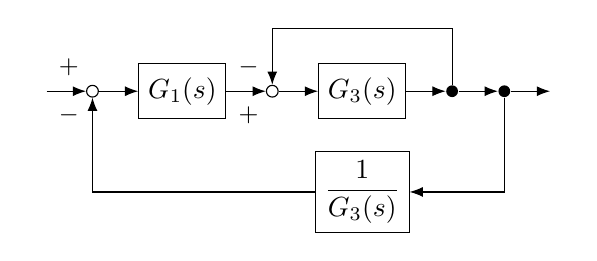
\begin{tikzpicture}[auto, node distance=0.3cm and 0.5cm, >=Latex]

  % --- 横並びノード配置 ---
  \node at (0,0) (input) {};
  \node[circle, draw, inner sep=1.5pt, right=of input] (sum1) {};               % 合流1
  \node[block, right=of sum1] (G1) {$G_1(s)$};
  \node[circle, draw, inner sep=1.5pt, right=of G1] (sum2) {};                  % 合流2
  \node[block, right=of sum2] (G3) {$G_3(s)$};
  \node[circle, fill=black, inner sep=1.5pt, right=of G3] (branch2) {};         % 分岐2(元の位置)
  \node[circle, fill=black, inner sep=1.5pt, right=of branch2] (branch1) {};    % 分岐1(右に移動)
  \node[right=of branch1] (output) {};

  % --- 1/G3ノード(下段) ---
  \node[block, below=0.4cm of G3] (invG3) {$\dfrac{1}{G_3(s)}$};

  % --- フィードバック座標(branch2 → sum2) ---
  \coordinate (fb2) at ($(branch2)+(0,0.8)$);

  % === 主系列 ===
  \draw[->] (input) -- (sum1);
  \draw[->] (sum1) -- (G1);
  \draw[->] (G1) -- (sum2);
  \draw[->] (sum2) -- (G3);
  \draw[->] (G3) -- (branch2);
  \draw[->] (branch2) -- (branch1);
  \draw[->] (branch1) -- (output);

  % === フィードバックルート1(branch1 → 1/G3 → sum1)===
  \draw[->] (branch1) |- (invG3);
  \draw[->] (invG3) -| (sum1);

  % === フィードバックルート2(branch2 → sum2)===
  \draw[->] (branch2) |- (fb2) -| (sum2);

  % --- 加算記号配置 ---
  \node at ($(sum1)+(-0.3,0.3)$) {\small $+$};
  \node at ($(sum1)+(-0.3,-0.3)$) {\small $-$};
  \node at ($(sum2)+(-0.3,0.3)$) {\small $-$};
  \node at ($(sum2)+(-0.3,-0.3)$) {\small $+$};

\end{tikzpicture}

\vspace{2mm}
    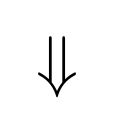
\begin{tikzpicture}
    \node {\Huge$\Downarrow$};
    \end{tikzpicture}
\vspace{2mm}



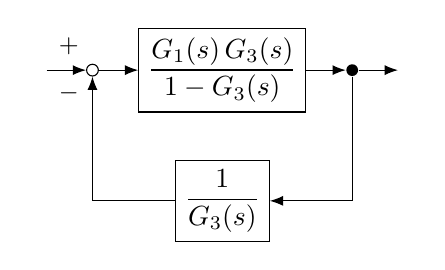
\begin{tikzpicture}[auto, node distance=0.3cm and 0.5cm, >=Latex]

  % --- 横並びノード配置 ---
  \node at (0,0) (input) {};
  \node[circle, draw, inner sep=1.5pt, right=of input] (sum1) {};                     % 合流点
  \node[block, right=of sum1] (G13series) {$\dfrac{G_1(s)\,G_3(s)}{1 - G_3(s)}$};     % 直列合成済
  \node[circle, fill=black, inner sep=1.5pt, right=of G13series] (branch1) {};        % 分岐点
  \node[right=of branch1] (output) {};

  % --- フィードバック用ノード ---
  \node[block, below=0.6cm of G13series] (invG3) {$\dfrac{1}{G_3(s)}$};

  % --- 主系列 ---
  \draw[->] (input) -- (sum1);
  \draw[->] (sum1) -- (G13series);
  \draw[->] (G13series) -- (branch1);
  \draw[->] (branch1) -- (output);

  % --- フィードバック(branch1 → 1/G3 → sum1) ---
  \draw[->] (branch1) |- (invG3);
  \draw[->] (invG3) -| (sum1);

  % --- 加算記号 ---
  \node at ($(sum1)+(-0.3,0.3)$) {\small $+$};
  \node at ($(sum1)+(-0.3,-0.3)$) {\small $-$};

\end{tikzpicture}

\vspace{2mm}
    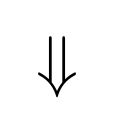
\begin{tikzpicture}
    \node {\Huge$\Downarrow$};
    \end{tikzpicture}
\vspace{2mm}


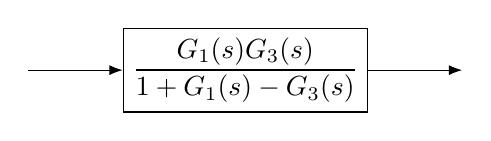
\begin{tikzpicture}[auto, node distance=1.5cm and 1.2cm, >=Latex]

  % --- ノード構成 ---
  \node[input] (input) {};
  \node[block, right=of input] (Gfinal) {$\dfrac{G_1(s) G_3(s)}{1 + G_1(s) - G_3(s)}$};
  \node[output, right=of Gfinal] (output) {};

  % --- 線描画 ---
  \draw[->] (input) -- (Gfinal);
  \draw[->] (Gfinal) -- (output);

\end{tikzpicture}




\end{center}

\vspace{-2mm}
よって、システム全体の伝達関数\(G_{All}(s)\)は
\vspace{-4mm}
\[
G_{All}(s) = \dfrac{G_1(s) G_3(s)}{1 + G_1(s) - G_3(s)}
\]


\end{tcolorbox}

\begin{tcolorbox}[title={1. (2)
    \vspace{-6mm}
    \begin{center}
        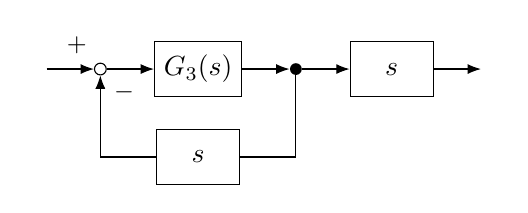
\begin{tikzpicture}[auto, node distance=0.4cm and 0.6cm, >=Latex]

        % --- 横並びの主系列ノード ---
        \node at (0,0) (input) {};
        \node[circle, draw, inner sep=1.5pt, right=of input] (sum) {};
        \node[block, right=of sum] (G3) {$G_3(s)$};
        \node[circle, fill=black, inner sep=1.5pt, right=of G3] (branch) {};
        \node[block, right=of branch] (s1) {$s$};
        \node[right=of s1] (output) {};
        
        % --- 下の s ノード ---
        \node[block, below=of G3] (s2) {$s$};
        
        % === 主系列 ===
        \draw[->] (input) -- (sum);
        \draw[->] (sum) -- (G3);
        \draw[->] (G3) -- (branch);
        \draw[->] (branch) -- (s1);
        \draw[->] (s1) -- (output);
        
        % === フィードバック経路(下) ===
        \draw[->] (branch) |- (s2) -| (sum);
        
        % --- 加算記号配置 ---
        \node at ($(sum)+(-0.3,0.3)$) {\small $+$};
        \node at ($(sum)+(0.3,-0.3)$) {\small $-$};
        
        \end{tikzpicture}
    \end{center} }]

    \begin{center}
        
        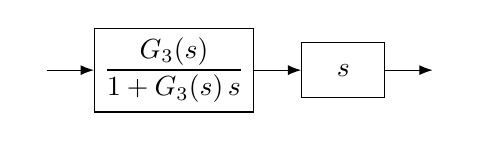
\begin{tikzpicture}[auto, node distance=0.4cm and 0.6cm, >=Latex]

        % --- ノード配置(フィードバック合成済・合流と分岐削除) ---
        \node at (0,0) (input) {};
        \node[block, right=of input] (Gfb) {$\dfrac{G_3(s)}{1 + G_3(s)\,s}$};
        \node[block, right=of Gfb] (s1) {$s$};
        \node[right=of s1] (output) {};

        % === 主系列 ===
        \draw[->] (input) -- (Gfb);
        \draw[->] (Gfb) -- (s1);
        \draw[->] (s1) -- (output);

        \end{tikzpicture}

        \vspace{2mm}
            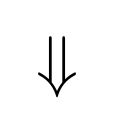
\begin{tikzpicture}
            \node {\Huge$\Downarrow$};
            \end{tikzpicture}
        \vspace{2mm}


        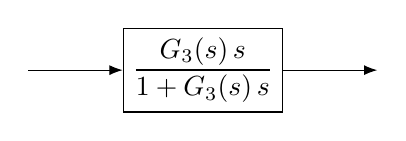
\begin{tikzpicture}[auto, node distance=1.5cm and 1.2cm, >=Latex]

        % --- ノード構成(完全合成) ---
        \node[input] (input) {};
        \node[block, right=of input] (Gfinal) {$\dfrac{G_3(s)\,s}{1 + G_3(s)\,s}$};
        \node[output, right=of Gfinal] (output) {};

        % --- 線描画 ---
        \draw[->] (input) -- (Gfinal);
        \draw[->] (Gfinal) -- (output);

        \end{tikzpicture}

    \end{center}

    \vspace{-2mm}
よって、システム全体の伝達関数\(G_{All}(s)\)は
\vspace{-4mm}
\[
G_{All}(s) = \dfrac{G_3(s)\,s}{1 + G_3(s)\,s}
\]

\end{tcolorbox}

\begin{tcolorbox}[title={1. (3)
    \vspace{-6mm}
    \begin{center}
        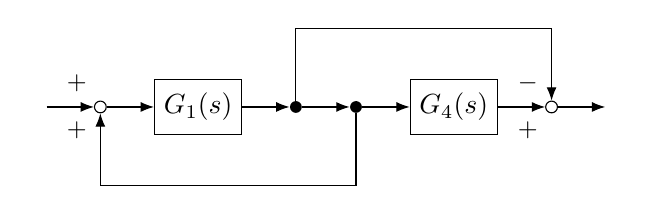
\begin{tikzpicture}[auto, node distance=0.4cm and 0.6cm, >=Latex]

            % --- 横並びノード ---
            \node at (0,0) (input) {};
            \node[circle, draw, inner sep=1.5pt, right=of input] (sum1) {};            % 合流1
            \node[block, right=of sum1] (G1) {$G_1(s)$};
            \node[circle, fill=black, inner sep=1.5pt, right=of G1] (branch1) {};      % 分岐1
            \node[circle, fill=black, inner sep=1.5pt, right=of branch1] (branch2) {}; % 分岐2
            \node[block, right=of branch2] (G4) {$G_4(s)$};
            \node[circle, draw, inner sep=1.5pt, right=of G4] (sum2) {};               % 合流2
            \node[right=of sum2] (output) {};
            
            % --- フィードバック座標 ---
            \coordinate (fb_down) at ($(branch2)+(0,-1.0)$);
            \coordinate (fb_up) at ($(branch1)+(0,1.0)$);
            
            % === 主系列 ===
            \draw[->] (input) -- (sum1);
            \draw[->] (sum1) -- (G1);
            \draw[->] (G1) -- (branch1);
            \draw[->] (branch1) -- (branch2);
            \draw[->] (branch2) -- (G4);
            \draw[->] (G4) -- (sum2);
            \draw[->] (sum2) -- (output);
            
            % === フィードバック経路 ===
            \draw[->] (branch2) |- (fb_down) -| (sum1);
            \draw[->] (branch1) |- (fb_up) -| (sum2);
            
            % --- 加算記号配置 ---
            \node at ($(sum1)+(-0.3,0.3)$) {\small $+$};
            \node at ($(sum1)+(-0.3,-0.3)$) {\small $+$};
            \node at ($(sum2)+(-0.3,0.3)$) {\small $-$};
            \node at ($(sum2)+(-0.3,-0.3)$) {\small $+$};
            
        \end{tikzpicture}
    \end{center}  }]

    \begin{center}
        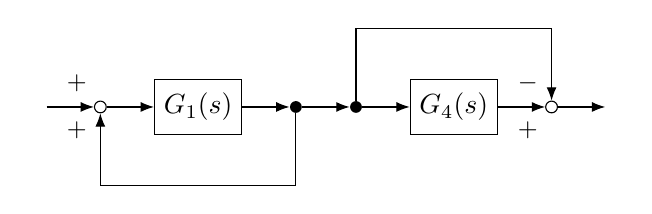
\begin{tikzpicture}[auto, node distance=0.4cm and 0.6cm, >=Latex]

        % --- 横並びノード(分岐1と分岐2の位置を入れ替え) ---
        \node at (0,0) (input) {};
        \node[circle, draw, inner sep=1.5pt, right=of input] (sum1) {};                  % 合流1
        \node[block, right=of sum1] (G1) {$G_1(s)$};
        \node[circle, fill=black, inner sep=1.5pt, right=of G1] (branch2) {};            % 分岐2(元:分岐1)
        \node[circle, fill=black, inner sep=1.5pt, right=of branch2] (branch1) {};       % 分岐1(元:分岐2)
        \node[block, right=of branch1] (G4) {$G_4(s)$};
        \node[circle, draw, inner sep=1.5pt, right=of G4] (sum2) {};                     % 合流2
        \node[right=of sum2] (output) {};

        % --- フィードバック座標 ---
        \coordinate (fb_down) at ($(branch2)+(0,-1.0)$);
        \coordinate (fb_up) at ($(branch1)+(0,1.0)$);

        % === 主系列 ===
        \draw[->] (input) -- (sum1);
        \draw[->] (sum1) -- (G1);
        \draw[->] (G1) -- (branch2);
        \draw[->] (branch2) -- (branch1);
        \draw[->] (branch1) -- (G4);
        \draw[->] (G4) -- (sum2);
        \draw[->] (sum2) -- (output);

        % === フィードバック経路(分岐位置入れ替えに従って接続) ===
        \draw[->] (branch2) |- (fb_down) -| (sum1);
        \draw[->] (branch1) |- (fb_up) -| (sum2);

        % --- 加算記号配置 ---
        \node at ($(sum1)+(-0.3,0.3)$) {\small $+$};
        \node at ($(sum1)+(-0.3,-0.3)$) {\small $+$};
        \node at ($(sum2)+(-0.3,0.3)$) {\small $-$};
        \node at ($(sum2)+(-0.3,-0.3)$) {\small $+$};

        \end{tikzpicture}

        \vspace{2mm}
            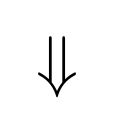
\begin{tikzpicture}
            \node {\Huge$\Downarrow$};
            \end{tikzpicture}
        \vspace{2mm}

        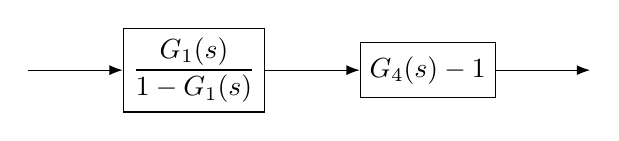
\begin{tikzpicture}[auto, node distance=1.8cm and 1.2cm, >=Latex]

        % --- 合成済みノード構成(G1と下段フィードバック、G4とsum2 合成済) ---
        \node[input] (input) {};
        \node[block, right=of input] (Gleft) {$\dfrac{G_1(s)}{1 - G_1(s)}$};          % G1と正帰還合成
        \node[block, right=of Gleft] (Gright) {$G_4(s) - 1$};                         % G4とsum2(−合流)合成
        \node[output, right=of Gright] (output) {};

        % --- 線描画 ---
        \draw[->] (input) -- (Gleft);
        \draw[->] (Gleft) -- (Gright);
        \draw[->] (Gright) -- (output);

        \end{tikzpicture}

        \vspace{2mm}
            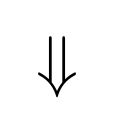
\begin{tikzpicture}
            \node {\Huge$\Downarrow$};
            \end{tikzpicture}
        \vspace{2mm}

        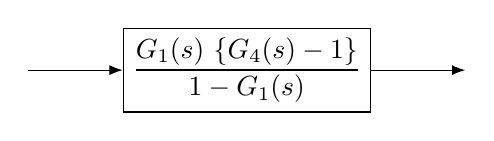
\begin{tikzpicture}[auto, node distance=2.0cm and 1.2cm, >=Latex]

        % --- 合成済みノード構成(完全合成) ---
        \node[input] (input) {};
        \node[block, right=of input] (Gfinal) 
            {$\displaystyle \frac{G_1(s)\,\left\{G_4(s) - 1\right\}}{1 - G_1(s)}$};
        \node[output, right=of Gfinal] (output) {};

        % --- 線描画 ---
        \draw[->] (input) -- (Gfinal);
        \draw[->] (Gfinal) -- (output);

        \end{tikzpicture}

    \end{center}
    よって、システム全体の伝達関数\(G_{All}(s)\)は
\[
G_{All}(s) = \dfrac{G_1(s)\,\left\{G_4(s) - 1\right\}}{1 - G_1(s)}
\]
\end{tcolorbox}

\begin{tcolorbox}[title={1. (4)
    \vspace{-6mm}
    \begin{center}
        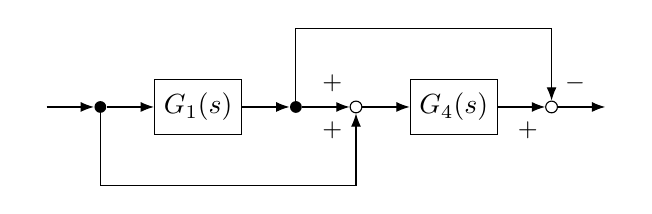
\begin{tikzpicture}[auto, node distance=0.4cm and 0.6cm, >=Latex]

        % --- 横並びノード(sum1 と branch2 の位置を交換) ---
        \node at (0,0) (input) {};
        \node[circle, fill=black, inner sep=1.5pt, right=of input] (branch2) {};     % ← 分岐2
        \node[block, right=of branch2] (G1) {$G_1(s)$};
        \node[circle, fill=black, inner sep=1.5pt, right=of G1] (branch1) {};        % 分岐1
        \node[circle, draw, inner sep=1.5pt, right=of branch1] (sum1) {};            % ← 合流1
        \node[block, right=of sum1] (G4) {$G_4(s)$};
        \node[circle, draw, inner sep=1.5pt, right=of G4] (sum2) {};                 % 合流2
        \node[right=of sum2] (output) {};
        
        % --- フィードバック座標 ---
        \coordinate (fb_down) at ($(branch2)+(0,-1.0)$);
        \coordinate (fb_up) at ($(branch1)+(0,1.0)$);
        
        % === 主系列 ===
        \draw[->] (input) -- (branch2);
        \draw[->] (branch2) -- (G1);
        \draw[->] (G1) -- (branch1);
        \draw[->] (branch1) -- (sum1);
        \draw[->] (sum1) -- (G4);
        \draw[->] (G4) -- (sum2);
        \draw[->] (sum2) -- (output);
        
        % === フィードバック経路 ===
        \draw[->] (branch2) |- (fb_down) -| (sum1);
        \draw[->] (branch1) |- (fb_up) -| (sum2);
        
        % --- 加算記号配置 ---
        \node at ($(sum1)+(-0.3,0.3)$) {\small $+$};
        \node at ($(sum1)+(-0.3,-0.3)$) {\small $+$};
        \node at ($(sum2)+(-0.3,-0.3)$) {\small $+$};
        \node at ($(sum2)+(0.3,0.3)$) {\small $-$};
        
        \end{tikzpicture}
    \end{center}  }]

    \begin{center}
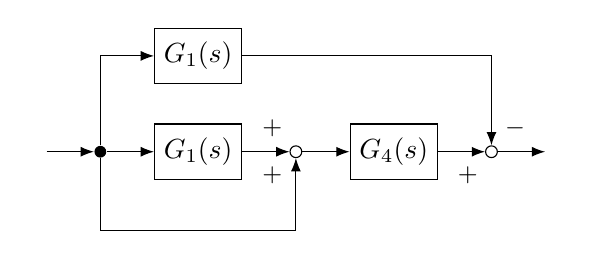
\begin{tikzpicture}[auto, node distance=0.4cm and 0.6cm, >=Latex]

% --- 横並びノード(分岐点を G1 の左に統一) ---
\node at (0,0) (input) {};
\node[circle, fill=black, inner sep=1.5pt, right=of input] (branch) {};           % 分岐点(統一)
\node[block, right=of branch] (G1) {$G_1(s)$};
\node[circle, draw, inner sep=1.5pt, right=of G1] (sum1) {};                      % 合流1
\node[block, right=of sum1] (G4) {$G_4(s)$};
\node[circle, draw, inner sep=1.5pt, right=of G4] (sum2) {};                      % 合流2
\node[right=of sum2] (output) {};

% --- 上ルートの追加ノード G₁(s) ---
\node[block, above=0.5cm of G1] (G1top) {$G_1(s)$};

% --- フィードバック座標(両方 branch 起点) ---
\coordinate (fb_down) at ($(branch)+(0,-1.0)$);
\coordinate (fb_up) at ($(branch)+(0,1.0)$);

% === 主系列 ===
\draw[->] (input) -- (branch);
\draw[->] (branch) -- (G1);
\draw[->] (G1) -- (sum1);
\draw[->] (sum1) -- (G4);
\draw[->] (G4) -- (sum2);
\draw[->] (sum2) -- (output);

% === 上ルート(branch → G1top → sum2)===
\draw[->] (branch) |- (G1top.west);
\draw[->] (G1top.east) -| (sum2.north);

% === フィードバック経路(そのまま) ===
\draw[->] (branch) |- (fb_down) -| (sum1);

% --- 加算記号配置 ---
\node at ($(sum1)+(-0.3,0.3)$) {\small $+$};
\node at ($(sum1)+(-0.3,-0.3)$) {\small $+$};
\node at ($(sum2)+(-0.3,-0.3)$) {\small $+$};
\node at ($(sum2)+(0.3,0.3)$) {\small $-$};

\end{tikzpicture}



    \vspace{2mm}
        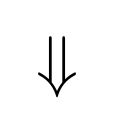
\begin{tikzpicture}
        \node {\Huge$\Downarrow$};
        \end{tikzpicture}
    \vspace{2mm}

    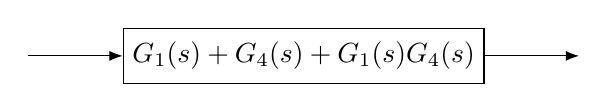
\begin{tikzpicture}[auto, node distance=2.0cm and 1.2cm, >=Latex]

    % --- 合成済みノード構成(完全伝達関数) ---
    \node[input] (input) {};
    \node[block, right=of input] (Gfinal) 
        {$ G_1(s) + G_4(s) + G_1(s)G_4(s)$};
    \node[output, right=of Gfinal] (output) {};

    % --- 線描画 ---
    \draw[->] (input) -- (Gfinal);
    \draw[->] (Gfinal) -- (output);

    \end{tikzpicture}

    \end{center}
\vspace{-4mm}
よって、システム全体の伝達関数\(G_{All}(s)\)は
\vspace{-2mm}
\[
G_{All}(s) = G_1(s) + G_4(s) + G_1(s)G_4(s)
\]
\end{tcolorbox}


% ---------------[2]--------------- 済
\begin{tcolorbox}[title={2.\quad \(\ddot{x}(t) - \sin(\omega t) = 0\) を解け。ただし、初期値はすべて0とする。
    }]
    \quad 両辺にラプラス変換を施すと,
    \vspace{-3mm}
    \begin{align*}
        &\qquad \mathcal{L}\left[ \ddot{x}(t) - \sin(\omega t) \right] 
        = 0 \\
        &\Leftrightarrow \left\{ s^2 X(s) - sx(0) - \dot{x}(0) \right\}
        - \frac{\omega}{s^2 + \omega^2}
        = 0  \\
        &\Leftrightarrow X(s) = \frac{\omega}{s^2(s^2 + \omega^2)}  \\
        &\Leftrightarrow X(s) = \frac{1}{\omega}\left\{\frac{1}{s^2} - \frac{1}{s^2 + \omega^2} \right\} 
    \end{align*}
    \vspace{-4mm}
    \quad 両辺にラプラス逆変換を施すと,
    \begin{align*}
    &\qquad \mathcal{L}^{-1} \left[ X(s) \right] 
    = \mathcal{L}^{-1} \left[ \frac{1}{\omega}\left\{\frac{1}{s^2} - \frac{1}{\omega} \frac{\omega}{s^2 + \omega^2} \right\}  \right] \\
    &\Leftrightarrow x(t) = \frac{1}{\omega} \left( t - \frac{1}{\omega} \sin \omega t \right)
    \end{align*}

\end{tcolorbox}

% ---------------[3]--------------- 済
\begin{tcolorbox}[title={3. 伝達関数\(\dfrac{s+1}{s^2+2s+4}\)のラプラス逆変換を行え。
    }]
    \vspace{-5mm}
\begin{align*}
    &\qquad G(s) =\frac{s+1}{s^2+2s+4}  \\
    &\Leftrightarrow G(s) =\frac{s + 1}{ ( s + 1 )^2+ 3} 
\end{align*}

\quad 両辺にラプラス逆変換を施すと,
\vspace{-3mm}
\begin{align*}
    &\qquad \mathcal{L}^{-1} \left[ G(s) \right] 
    =\mathcal{L}^{-1} \left[ \frac{s + 1}{ ( s + 1 )^2+ 3}  \right] \\
    &\Leftrightarrow g(t) = e^{-t} \cos (\sqrt{3} t)   
\end{align*}

\end{tcolorbox}



% ---------------[4]---------------
\noindent
\begin{minipage}[t]{0.005\linewidth}
    4.
\end{minipage}
\hfill
\begin{minipage}[t]{0.595\linewidth}
右図に示す系について、入力を変位\(x_1(t)\)、出力を変位\(x_2(t)\)としたとき、
次の問いに答えよ。なお、\(m\)は質量[kg]、\(d\)は粘性係数[Ns/m]、
\(k_1\)、\(k_2\)はバネ[N/m] 
とし、初期状態において系は静止しているとする。  
\end{minipage}
\hfill
\begin{minipage}[t]{0.35\linewidth}
    \vspace{-6mm}
    \begin{center}
        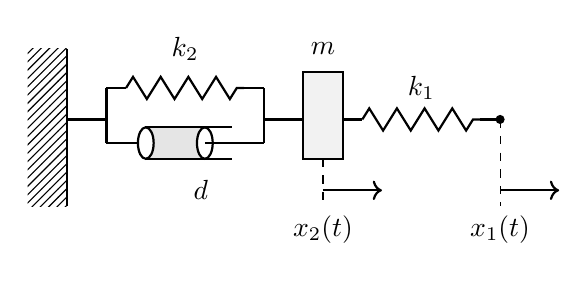
\begin{tikzpicture}[scale=1.0]
          % 固定壁
          \fill[pattern=north east lines] (-1,0,0) rectangle (-0.5,2);
          \draw[thick] (-0.5,0) -- (-0.5,2);
      
          %接続部1
          \draw[thick] (-0.5,1.1) -- (0,1.1);
          \draw[thick] (0,0.8) -- (0,1.5);
        
          % バネ2
          \draw[thick] (0,1.5) -- (0.25,1.5);
          \draw[thick, decorate, decoration={zigzag, segment length=10, amplitude=4}] (0.25,1.5) -- (1.75,1.5);
          \draw[thick] (1.75,1.5) -- (2.0,1.5);
          \node at (1.0,2.0) {$k_2$};
        
          % ダンパー(シリンダー形式)
          \draw[thick] (0,0.8) -- (0.5,0.8); % 棒
          \draw[thick, fill=gray!20] (0.5,0.6) rectangle (1.25,1.0); % 筒の側面
          \draw[thick] (1.25,1.0) -- (1.60,1.0); % 筒の上
          \draw[thick] (1.25,0.6) -- (1.60,0.6); % 筒の下
          \draw[thick, fill=white] (0.5,0.8) ellipse (0.1 and 0.2); % 左端面
          \draw[thick, fill=white] (1.25,0.8) ellipse (0.1 and 0.2); % 右端面
          \draw[thick] (1.25,0.8) -- (2.0,0.8); % ピストン棒
          \node at (1.2,0.2) {$d$};
      
          %接続部2
          \draw[thick] (2.0,0.8) -- (2.0,1.5);
          \draw[thick] (2.0,1.1) -- (2.5,1.1);
        
          % 質量M
          \draw[thick, fill=gray!10] (2.5,0.6) rectangle (3.0,1.7);
          \node at (2.75,2.0) {$m$};
      
          % バネ1
          \draw[thick] (3.0,1.1) -- (3.25,1.1);
          \draw[thick, decorate, decoration={zigzag, segment length=10, amplitude=4}] (3.25,1.1) -- (4.75,1.1);
          \draw[thick] (4.75,1.1) -- (5.0,1.1);
          \node at (4.0,1.5) {$k_1$};
      
          % 丸
          \draw[fill] (5,1.1) circle (0.05);
      
        
          % 座標x1
          \draw[->, thick] (5,0.2) -- (5.75,0.2);
          \node at (5,-0.3) {$x_1(t)$};
          \draw[dashed] (5,1.1) -- (5,0);
      
          % 座標x2
          \draw[->, thick] (2.75,0.2) -- (3.5,0.2);
          \node at (2.75,-0.3) {$x_2(t)$};
          \draw[dashed] (2.75,0.6) -- (2.75,0);
        
        \end{tikzpicture}
    \end{center}
\end{minipage}\\

\indent
(1)この図によって示されるシステムの運動方程式と伝達関数を求めよ。\\

\indent
(2)\(m=1,d=4,k_1=1,k_2=2\)とし、インパルス応答、ステップ応答をそれぞれ求\\
\indent \quad めよ。\\

\indent
(3)\(m=1,d=2,k_1=3,k_2=2\)とし、ステップ応答を求めよ。\\

\indent
(4)\(m=1,d=2,k_1=1,k_2=0\)とし、ステップ応答を求めよ。\\

\indent
(5)\(m=1,d=0,k_1=1,k_2=2\)とし、ステップ応答を求めよ。\\

\indent
(6)\(m=1,d=0,k_1=2,k_2=1\)とし、入力変位\(x_1(t)=\sin(t)\)を与えたときの応答を求
\indent \quad めよ。\\

\indent
(7)\(m=1,d=2,k_1=1,k_2=1\)とし、入力変位\(x_1(t)=\sin(2t)\)を与えたときの応答を
\indent \quad 求めよ。\\

% ---------------[4(1)]--------------- 済
\begin{tcolorbox}[title={4. (1)この図によって示されるシステムの運動方程式と伝達関数を求めよ。 
    }]

    \(x(t)\)に関する運動方程式は
    \begin{align*}
        &\qquad m\ddot{x}_2 =-k_2 x_2 - d \dot{x}_2 - k_1 \left(x_2 - x_1\right) \\
    \end{align*}
    また伝達関数は
    \begin{align*}
        &\qquad m\ddot{x}_2 +  d \dot{x}_2 + \left(k_1+k_2\right) x_2
        = k_1 x_1 \\
        &\therefore \quad \mathcal{L} \left[ m\ddot{x}_2 +  d \dot{x}_2 + \left(k_1+k_2\right) x_2\right] 
        =\mathcal{L} \left[ k_1 x_1 \right] \\
        &\therefore \quad \left\{m s^2 + d s + \left(k_1+k_2\right) \right\}\,X_2(s) = k_1 X_1(s) \quad [\because \dot{x}(0)=x(0)=0 ]\\
        &\therefore \quad G(s) \;=\;\frac{X_2(s)}{X_1(s)}
        \;=\;\frac{k_1}{m s^2 + d s + \left(k_1 + k_2\right)}
    \end{align*}

\end{tcolorbox}

% ---------------[4(2)]--------------- 済
\begin{tcolorbox}[title={4. (2)\(m=1,d=4,k_1=1,k_2=2\)とし、インパルス応答、ステップ応答をそれぞれ\\
\indent \quad 求めよ。}]

    (\uppercase\expandafter{\romannumeral 1})インパルス応答 \\
    パラメータを代入し、インパルス入力のラプラス変換は\(F(s)=1\)なので
    \vspace{-2mm}
    \begin{align*}
        &\qquad G(s) = \frac{1}{s^2 + 4 s + 3 } \\
        &\therefore \quad X(s) = G(s) F(s) = \frac{1}{(s+1)(s+3)} \\
        &\therefore \quad X(s) = \frac{1}{2} \left( \frac{1}{s+1} + \frac{-1}{s+3} \right)\\
        &\therefore \quad \mathcal{L}^{-1} \left[ X(s)\right] 
        =\frac{1}{2} \left\{ \mathcal{L}^{-1} \left[\frac{1}{s+1}\right] 
        + \mathcal{L}^{-1} \left[\frac{-1}{s+3}\right] \right\}\\
        &\therefore \quad x(t) = \frac{1}{2}\left(e^{-t} - e^{-3t} \right)
    \end{align*}

    (\uppercase\expandafter{\romannumeral 2})ステップ応答 \\
    パラメータを代入し、ステップ入力のラプラス変換は\(F(s)=\dfrac{1}{s}\)なので
    \vspace{-2mm}
    \begin{align*}
        &\qquad G(s) = \frac{1}{s^2 + 4 s + 3 } \\
        &\therefore \quad X(s) = G(s) F(s) = \frac{1}{s(s+1)(s+3)} \\
        &\therefore \quad X(s) = \frac{\frac{1}{3}}{s} 
        + \frac{\left(-\frac{1}{2}\right)}{s+1} 
        + \frac{\left(\frac{1}{6}\right)}{s+3} \\
        &\therefore \quad \mathcal{L}^{-1} \left[ X(s)\right] 
        = \mathcal{L}^{-1} \left[\frac{\left(\frac{1}{3}\right)}{s}\right] 
        + \mathcal{L}^{-1} \left[\frac{\left(-\frac{1}{2}\right)}{s+1}\right]
        + \mathcal{L}^{-1} \left[\frac{\left(\frac{1}{6}\right)}{s+3}\right] \\
        &\therefore \quad x(t) = \frac{1}{3} - \frac{1}{2}e^{-t} +\frac{1}{6} e^{-3t}
    \end{align*}

\end{tcolorbox}

% ---------------[4(3)]--------------- 済
\begin{tcolorbox}[title={4. (3)\(m=1,d=2,k_1=3,k_2=2\)とし、ステップ応答を求めよ。 
    }]
    パラメータを代入し、ステップ入力のラプラス変換は\(F(s)=\dfrac{1}{s}\)なので
    \vspace{-4mm}
    \begin{align*}
        &\qquad G(s) = \frac{3}{s^2 + 2s + 5 } \\
        &\therefore \quad X(s) = G(s) F(s) 
        = \frac{3}{s(s^2 + 2s + 5)} \\
        &\therefore \quad X(s) = \frac{\left(\frac{3}{5}\right)}{s}
        +\frac{-\frac{3}{5}s-\frac{6}{5}}{s^2 + 2s + 5} \\
        &\therefore \quad \mathcal{L}^{-1} \left[ X(s)\right] 
        = \mathcal{L}^{-1} \left[\frac{\left(\frac{3}{5}\right)}{s}\right] 
        + \mathcal{L}^{-1} \left[\frac{-\frac{3}{5}\left\{(s+1)+\frac{1}{2}\cdot 2\right\}}{\left(s+1\right)^2+2^2} \right] \\
        &\therefore \quad x(t) = \frac{3}{5} -\frac{3}{5} e^{-t} \left\{ \cos 2t + \frac{1}{2} \sin 2t\right\}
    \end{align*}

\end{tcolorbox}

% ---------------[4(4)]--------------- 済
\begin{tcolorbox}[title={4. (4)\(m=1,d=2,k_1=1,k_2=0\)とし、ステップ応答を求めよ。 
    }]
    パラメータを代入し、ステップ入力のラプラス変換は\(F(s)=\dfrac{1}{s}\)なので
    \vspace{-4mm}
    \begin{align*}
        &\qquad G(s) = \frac{1}{s^2 + 2s + 1} \\
        &\therefore \quad X(s) = G(s) F(s) = \frac{1}{s(s+1)^2} \\
        &\therefore \quad X(s) = \frac{1}{s}+\frac{-1}{(s+1)^2}+\frac{-1}{s+1} \\
        &\therefore \quad \mathcal{L}^{-1} \left[ X(s)\right] 
        = \mathcal{L}^{-1} \left[\frac{1}{s}\right] 
        + \mathcal{L}^{-1} \left[\frac{-1}{(s+1)^2} \right]
        + \mathcal{L}^{-1} \left[\frac{-1}{s+1} \right] \\
        &\therefore \quad x(t) = 1 - e^{-t}(t+1)
    \end{align*}

\end{tcolorbox}

% ---------------[4(5)]--------------- 済
\begin{tcolorbox}[title={4. (5)\(m=1,d=0,k_1=1,k_2=2\)とし、ステップ応答を求めよ。 
    }]
    パラメータを代入し、ステップ入力のラプラス変換は\(F(s)=\dfrac{1}{s}\)なので
    \vspace{-4mm}
    \begin{align*}
        &\qquad G(s) = \frac{1}{s^2 + 3} \\
        &\therefore \quad X(s) = G(s) F(s) = \frac{1}{s(s^2+3)} \\
        &\therefore \quad X(s) = \frac{\left(\frac{1}{3}\right)}{s}
        + \frac{\left(-\frac{1}{3}s\right)}{s^2+3} \\
        &\therefore \quad \mathcal{L}^{-1} \left[ X(s)\right] 
        = \mathcal{L}^{-1} \left[\frac{\left(\frac{1}{3}\right)}{s}\right] 
        + \mathcal{L}^{-1} \left[\frac{\left(-\frac{1}{3}s\right)}{s^2+3} \right] \\
        &\therefore \quad x(t) = \frac{1}{3} - \frac{1}{3}  \cos \left( \sqrt{3} t \right)
    \end{align*}

\end{tcolorbox}


% ---------------[4(6)]--------------- 済
\begin{tcolorbox}[title={4. (6)\(m=1,d=0,k_1=2,k_2=1\)とし、入力変位\(x_1(t)=\sin(t)\)を与えたときの応
\indent \quad 答を求めよ。 }]
パラメータを代入し、\(x_1(t)=\sin(t)\)のラプラス変換は\(X_i(s)=\dfrac{1}{s^2+1}\)なので
    \vspace{-4mm}
    \begin{align*}
        &\qquad G(s) = \frac{2}{s^2 +3} \\
        &\therefore \quad X(s) = G(s) F(s) = \frac{2}{(s^2 +1)(s^2+3)} \\
        &\therefore \quad X(s) =  \frac{1}{s^2 +1}
        + \frac{(-1)}{s^2+3}\\
        &\therefore \quad \mathcal{L}^{-1} \left[ X(s)\right] 
        = \mathcal{L}^{-1} \left[\frac{1}{s^2 +1} \right]
        - \frac{1}{\sqrt{3}} \cdot \mathcal{L}^{-1} \left[\frac{\sqrt{3}}{s^2+3} \right] \\
        &\therefore \quad x(t) = \sin t - \frac{1}{\sqrt{3}} \sin (\sqrt{3}t)
    \end{align*}
\end{tcolorbox}

% ---------------[4(7)]--------------- 済
\begin{tcolorbox}[title={4. (7)\(m=1,d=2,k_1=1,k_2=1\)とし、入力変位\(x_1(t)=\sin(2t)\)を与えたときの応
\indent \quad 答を求めよ。 }]
パラメータを代入し、\(x_1(t)=\sin(2t)\)のラプラス変換は\(X_i(s)=\dfrac{2}{s^2+2^2}\)なので
    \vspace{-4mm}
    \begin{align*}
        &\qquad G(s) = \frac{1}{s^2 + 2s+ 1} \\
        &\therefore \quad X(s) = G(s) F(s) = \frac{1}{(s+1)^2(s^2+2^2)} \\
        &\therefore \quad X(s) =  \frac{\left(\frac{1}{5}\right)}{(s+1)^2} 
        + \frac{\left(\frac{2}{25}\right)}{s+1}
        + \frac{\left(-\frac{2}{25}s-\frac{3}{25}\right)}{s^2+2^2}\\
        &\therefore \quad \mathcal{L}^{-1} \left[ X(s)\right] 
        = \mathcal{L}^{-1} \left[\frac{\left(\frac{5}{25}\right)}{(s+1)^2}  \right]
        + \mathcal{L}^{-1} \left[\frac{\left(\frac{2}{25}\right)}{s+1} \right]
        + \mathcal{L}^{-1} \left[\frac{\left(-\frac{2}{25}s-\frac{3}{25}\right)}{s^2+2^2}\right]  \\
        &\therefore \quad x(t) = \frac{1}{25}e^{-t}(5t+2)- \frac{1}{25}\left(2\cos 2t + \frac{3}{2}\sin 2t\right)
    \end{align*}
\end{tcolorbox}


\newpage

% ---------------[5]---------------
\noindent
\begin{minipage}[t]{0.005\linewidth}
    5.
\end{minipage}
\hfill
\begin{minipage}[t]{0.595\linewidth}
右図に示す系について、入力を変位\(x_1(t)\)、出力を変位\(x_2(t)\)としたとき、
次の問いに答えよ。なお、\(m\)は質量[kg]、\(d\)は粘性係数[Ns/m]、
\(k_1\)、\(k_2\)はバネ[N/m] 
とし、初期状態において系は静止しているとする。  
\end{minipage}
\hfill
\begin{minipage}[t]{0.35\linewidth}
    \vspace{-6mm}
    \begin{center}
        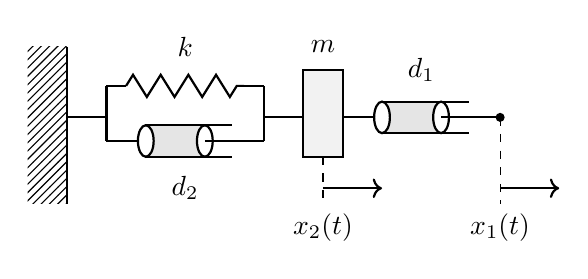
\begin{tikzpicture}[scale=1.0]
          % 固定壁
          \fill[pattern=north east lines] (-1,0,0) rectangle (-0.5,2);
          \draw[thick] (-0.5,0) -- (-0.5,2);
      
          %接続部1
          \draw[thick] (-0.5,1.1) -- (0,1.1);
          \draw[thick] (0,0.8) -- (0,1.5);
        
          % バネ1
          \draw[thick] (0,1.5) -- (0.25,1.5);
          \draw[thick, decorate, decoration={zigzag, segment length=10, amplitude=4}] (0.25,1.5) -- (1.75,1.5);
          \draw[thick] (1.75,1.5) -- (2.0,1.5);
          \node at (1.0,2.0) {$k$};
        
          % ダンパー2(シリンダー形式)
          \draw[thick] (0,0.8) -- (0.5,0.8); % 棒
          \draw[thick, fill=gray!20] (0.5,0.6) rectangle (1.25,1.0); % 筒の側面
          \draw[thick] (1.25,1.0) -- (1.60,1.0); % 筒の上
          \draw[thick] (1.25,0.6) -- (1.60,0.6); % 筒の下
          \draw[thick, fill=white] (0.5,0.8) ellipse (0.1 and 0.2); % 左端面
          \draw[thick, fill=white] (1.25,0.8) ellipse (0.1 and 0.2); % 右端面
          \draw[thick] (1.25,0.8) -- (2.0,0.8); % ピストン棒
          \node at (1.0,0.2) {$d_2$};
      
          %接続部2
          \draw[thick] (2.0,0.8) -- (2.0,1.5);
          \draw[thick] (2.0,1.1) -- (2.5,1.1);
        
          % 質量M
          \draw[thick, fill=gray!10] (2.5,0.6) rectangle (3.0,1.7);
          \node at (2.75,2.0) {$m$};
      
          % ダンパー1(シリンダー形式)
          \draw[thick] (3,1.1) -- (3.5,1.1); % 棒
          \draw[thick, fill=gray!20] (3.5,0.9) rectangle (4.25,1.3); % 筒の側面
          \draw[thick] (4.25,1.3) -- (4.60,1.3); % 筒の上
          \draw[thick] (4.25,0.9) -- (4.60,0.9); % 筒の下
          \draw[thick, fill=white] (3.5,1.1) ellipse (0.1 and 0.2); % 左端面
          \draw[thick, fill=white] (4.25,1.1) ellipse (0.1 and 0.2); % 右端面
          \draw[thick] (4.25,1.1) -- (5,1.1); % ピストン棒
          \node at (4.0,1.7) {$d_1$};
      
          % 丸
          \draw[fill] (5,1.1) circle (0.05);
      
        
          % 座標x1
          \draw[->, thick] (5,0.2) -- (5.75,0.2);
          \node at (5,-0.3) {$x_1(t)$};
          \draw[dashed] (5,1.1) -- (5,0);
      
          % 座標x2
          \draw[->, thick] (2.75,0.2) -- (3.5,0.2);
          \node at (2.75,-0.3) {$x_2(t)$};
          \draw[dashed] (2.75,0.6) -- (2.75,0);
        
        \end{tikzpicture}
    \end{center}
\end{minipage}\\

\indent
(1)この図によって示されるシステムの運動方程式と伝達関数を求めよ。\\

\indent
(2)\(x_1(t)\)に単位ステップ入力を印加した際の応答について、\(x_2(t)\)の定常値を求めよ。\\

\indent
(3)\(m=1,d_1=1,d_2=1,k=1\)としインパルス応答,ステップ応答をそれぞれ求めよ。\\

\indent
(4)\(m=1,d_1=2,d_2=2,k=5\)とし、ステップ応答を求めよ。\\

\indent
(5)\(m=d_1=d_2=k=1\)とし、入力\(x_1(t)=\sin(t)\)を与えたときの応答を求めよ。\\

\indent
(6)\(m=d_1=1,d_2=k=2\)とし、入力\(x_1(t)=\sin(2t)\)を与えたときの応答を求めよ。\\

\indent
(7)\(m=1,d_1=2,d_2=0,k=2\)とし、ステップ応答を求めよ。

% ---------------[5(1)]--------------- 済
\begin{tcolorbox}[title={5. (1)この図によって示されるシステムの運動方程式と伝達関数を求めよ。 
    }]

    \(x(t)\)に関する運動方程式は
    \vspace{-4mm}
    \begin{align*}
        &\qquad m\ddot{x}_2 =-k x_2 - d_2 \dot{x}_2 - d_1 \left(\dot{x}_2 - \dot{x}_1\right) 
    \end{align*}
    \vspace{-4mm}
    また伝達関数は
    \begin{align*}
        &\qquad m\ddot{x}_2 +  (d_1+d_2) \dot{x}_2 + k x_2
        = d_1 \dot{x}_1 \\
        &\therefore \quad \mathcal{L} \left[m\ddot{x}_2 +  (d_1+d_2) \dot{x}_2 + k x_2\right] 
        =\mathcal{L} \left[d_1 \dot{x}_1 \right] \\
        &\therefore \quad \left\{m s^2 +(d_1+d_2) s + k \right\}\,X_2(s) = d_1 s  X_1(s) \quad [\because \dot{x}(0)=x(0)=0 ]\\
        &\therefore \quad G(s) \;=\;\frac{X_2(s)}{X_1(s)}
        \;=\;\frac{d_1 s}{m s^2 +(d_1+d_2) s + k}
    \end{align*}
\end{tcolorbox}

% ---------------[5(2)]--------------- 済
\begin{tcolorbox}[title={5. (2)\(x_1(t)\)に単位ステップ入力を印加した際の応答について、\(x_2(t)\)の定常値を求めよ。 
    }]

            ステップ入力のラプラス変換は\(X_1(s)=\frac{1}{s}\)なので
    \vspace{-4mm}
    \begin{align*}
        &\qquad G(s) = \frac{d_1 s}{m s^2 +(d_1+d_2) s + k} \\
        &\therefore \quad X_o(s) = G(s) X_i(s) = \frac{d_1}{m s^2 +(d_1+d_2) s + k}
    \end{align*}
    最終値定理より
    \vspace{-4mm}
    \begin{align*}
    \lim_{t \to \infty} x_o(t) &= \lim_{s \to 0} sX_o(s) \\
        &= \lim_{s \to 0} \frac{d_1 s}{m s^2 +(d_1+d_2) s + k} \\
        &= 0
    \end{align*}
\end{tcolorbox}

% ---------------[5(3)]--------------- 済
\begin{tcolorbox}[title={5. (3)\(m=1,d_1=1,d_2=1,k=1\)とし、インパルス応答、ステップ応答をそれぞれ\\
\indent \quad 求めよ。}]

(\uppercase\expandafter{\romannumeral 1})インパルス応答 \\
    パラメータを代入し、インパルス入力のラプラス変換は\(F(s)=1\)なので
    \vspace{-2mm}
    \begin{align*}
        &\qquad G(s) = \frac{s}{s^2 + 2 s + 1 } \\
        &\therefore \quad X(s) = G(s) F(s) = \frac{s}{(s+1)^2} \\
        &\therefore \quad X(s) = \frac{-1}{(s+1)^2} + \frac{1}{s+1} \\
        &\therefore \quad \mathcal{L}^{-1} \left[ X(s)\right] 
        =\mathcal{L}^{-1} \left[\frac{-1}{(s+1)^2}\right] 
        + \mathcal{L}^{-1} \left[\frac{1}{s+1}\right] \\
        &\therefore \quad x(t) = - e^{-t} (t-1) 
    \end{align*}

    (\uppercase\expandafter{\romannumeral 2})ステップ応答 \\
    パラメータを代入し、ステップ入力のラプラス変換は\(F(s)=\dfrac{1}{s}\)なので
    \vspace{-2mm}
    \begin{align*}
        &\qquad G(s) = \frac{s}{s^2 + 2 s + 1 } \\
        &\therefore \quad X(s) = G(s) F(s) = \frac{1}{(s+1)^2} \\
        &\therefore \quad \mathcal{L}^{-1} \left[ X(s)\right] 
        =\mathcal{L}^{-1} \left[\frac{1}{(s+1)^2}\right] \\
        &\therefore \quad x(t) = te^{-t} 
    \end{align*}

\end{tcolorbox}

% ---------------[5(4)]--------------- 済
\begin{tcolorbox}[title={5. (4)\(m=1,d_1=2,d_2=2,k=5\)とし、ステップ応答を求めよ。 }]

    パラメータを代入し、ステップ入力のラプラス変換は\(F(s)=\dfrac{1}{s}\)なので
    \vspace{-4mm}
    \begin{align*}
        &\qquad G(s) = \frac{2s}{s^2 + 4s + 5 } \\
        &\therefore \quad X(s) = G(s) F(s) 
        = \frac{2}{(s+2)^2+1^2} \\
        &\therefore \quad \mathcal{L}^{-1} \left[ X(s)\right] 
        = \mathcal{L}^{-1} \left[\frac{2}{(s+2)^2+1^2}\right] \\
        &\therefore \quad x(t) = 2e^{-2t} \sin t
    \end{align*}

\end{tcolorbox}

% ---------------[5(5)]--------------- 済
\begin{tcolorbox}[title={5. (5)\(m=1,d_1=1,d_2=1,k=1\)とし、入力変位\(x_1(t)=\sin(t)\)を与えたときの応
\indent \quad 答を求めよ。 }]

パラメータを代入し、\(x_1(t)=\sin(t)\)のラプラス変換は\(X_i(s)=\dfrac{1}{s^2+1}\)なので
    \vspace{-4mm}
    \begin{align*}
        &\qquad G(s) = \frac{s}{s^2 + 2s + 1} \\
        &\therefore \quad X(s) = G(s) F(s) = \frac{s}{(s+1)^2(s^2 +1)} \\
        &\therefore \quad X(s) =  \frac{\left(-\frac{1}{2}\right)}{(s+1)^2}
        + \frac{\left(\frac{1}{2}\right)}{s^2 +1}\\
        &\therefore \quad \mathcal{L}^{-1} \left[ X(s)\right] 
        = \mathcal{L}^{-1} \left[\frac{\left(-\frac{1}{2}\right)}{(s+1)^2}\right]
        + \mathcal{L}^{-1} \left[\frac{\left(\frac{1}{2}\right)}{s^2 +1}\right] \\
        &\therefore \quad x(t) = -\frac{1}{2} t e^{-t} + \frac{1}{2} \sin t
    \end{align*}

\end{tcolorbox}

% ---------------[5(6)]--------------- 済
\begin{tcolorbox}[title={5. (6)\(m=1,d_1=1,d_2=2,k=2\)とし、入力変位\(x_1(t)=\sin(2t)\)を与えたときの応
\indent \quad 答を求めよ。 }]

パラメータを代入し、\(x_1(t)=\sin(2t)\)のラプラス変換は\(X_i(s)=\dfrac{2}{s^2+2^2}\)なので
    \vspace{-4mm}
    \begin{align*}
        &\qquad G(s) = \frac{s}{s^2 + 3s + 2} \\
        &\therefore \quad X(s) = G(s) F(s) = \frac{s}{(s+1)(s+2)(s^2+2^2)} \\
        &\therefore \quad X(s) =  \frac{\left(-\frac{1}{5}\right)}{s+1} 
        + \frac{\left(\frac{1}{4}\right)}{s+2}
        + \frac{\left(-\frac{1}{20}s+\frac{3}{10}\right)}{s^2+2^2}\\
        &\therefore \quad \mathcal{L}^{-1} \left[ X(s)\right] 
        = \mathcal{L}^{-1} \left[\frac{\left(-\frac{1}{5}\right)}{s+1}  \right]
        + \mathcal{L}^{-1} \left[\frac{\left(\frac{1}{4}\right)}{s+2} \right]
        + \mathcal{L}^{-1} \left[\frac{\left(-\frac{1}{20}s+\frac{3}{10}\right)}{s^2+2^2}\right]  \\
        &\therefore \quad x(t) = -\frac{1}{5} e^{-t} + \frac{1}{4} e^{-2t} - \frac{1}{20} \left\{ \cos (2t) - 3\sin (2t)\right\}
    \end{align*}

\end{tcolorbox}

% ---------------[5(7)]--------------- 済
\begin{tcolorbox}[title={5. (7)\(m=1,d_1=2,d_2=0,k=2\)とし、ステップ応答を求めよ。 }]

    パラメータを代入し、ステップ入力のラプラス変換は\(F(s)=\dfrac{1}{s}\)なので
    \vspace{-4mm}
    \begin{align*}
        &\qquad G(s) = \frac{2s}{s^2 + 2s + 2} \\
        &\therefore \quad X(s) = G(s) F(s) 
        = \frac{2}{s^2 + 2s + 2} \\
        &\therefore \quad \mathcal{L}^{-1} \left[ X(s)\right] 
        = \mathcal{L}^{-1} \left[\frac{2}{(s+1)^2+1}\right] \\
        &\therefore \quad x(t) = 2 e^{-t} \sin t
    \end{align*}

\end{tcolorbox}

% ---------------[6]--------------- 
\begin{tcolorbox}[title={6. 伝達関数\(G_1(s)=\dfrac{1}{s+0.1}\)について漸近線を用いてボード線図を描け。
まず\(10 \times \dfrac{1}{10s+1}\)として一次遅れ系に変形した上で、
ゲイン(dB)、位相(deg.)を求めよ。各軸には適宜数値を記入し、
折れ点等の特徴点を明示すること。}]

ゲイン[dB]は\(20\log_{10} \left| G(j\omega) \right|\)で表されるので\\
\vspace{-6mm}
\begin{align*}
    G(j\omega) &= \frac{10}{10j \omega + 1} \\
    \therefore \quad \left| G(j\omega) \right| 
    &= \left| \frac{10}{10j \omega + 1} \right| 
    =  \frac{10}{\sqrt{(10\omega)^2 + 1}} 
\end{align*}
よってゲイン[dB]は\\
\vspace{-6mm}
\begin{align*}
dB &= 20 \log_{10} \left( \frac{10}{\sqrt{(10\omega)^2 + 1}} \right) = 20 - 20 \log_{10} \left( \frac{1}{\sqrt{(10\omega)^2 + 1}} \right)
\end{align*}

位相は\angle G(j\omega)で与えられるので、

\[
G(j\omega) = 10 \times \frac{10 j \omega - 1}{(10\omega)^2 + 1} \\
\]

であることに注意して分子に着目すると、実部が\(-1\)、虚部が\(10 \omega \)なので下図より\\

\begin{minipage}{0.45\linewidth}
\vspace{-9mm}
\begin{align*}
    \angle G(j\omega) &= \pi - \tan^{-1}(10\omega) 
\end{align*}
    定義域  \( -\dfrac{\pi}{2} < \angle G(j\omega) < \dfrac{\pi}{2} \) より
\begin{align*}
    \angle G(j\omega) &= -\tan^{-1}(10\omega)
\end{align*}
\end{minipage}
\hfill
\begin{minipage}{0.5\linewidth}
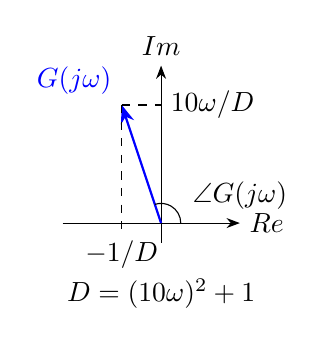
\begin{tikzpicture}[>=Stealth, scale=0.5]

  % 軸
  \draw[->] (-2.5, 0) -- (2, 0) node[right] {$Re$};
  \draw[->] (0, -0.5) -- (0, 4) node[above] {$Im$};

  % ベクトルの終点(実部 -1, 虚部 3)
  \coordinate (P) at (-1, 3);

  % ベクトル G(jω)
  \draw[thick, blue, ->] (0, 0) -- (P) node[above left] {$G(j\omega)$};

  % 補助線
  \draw[dashed] (P) -- (-1, -0.2) node[below] {$-1 / D$};
  \draw[dashed] (P) -- (0, 3) node[right] {$10\omega / D$};

  % 角度(偏角θ)
  \draw (0.5, 0) arc[start angle=0, end angle=108.4, radius=0.5cm];
  \node at (2.0, 0.7) {$\angle G(j\omega)$};

  % 注記
  \node at (0, -1.8) {$ D = (10\omega)^2 + 1$};

\end{tikzpicture}
\end{minipage}

\begin{minipage}{0.45\linewidth}
また、ボード線図は\\
\(\omega >> 1\) のとき
\[
dB = 20 -   20 \log_{10} \left( \dfrac{1}{10\omega} \right) 
\]  
\(\omega << 1\) のとき
\[
dB = 20
\]   
\end{minipage}
\hfill
\begin{minipage}{0.5\linewidth}
    \begin{center}
\begin{tikzpicture}[scale=0.3,xscale=4.2, yscale=0.05]

  % 軸
  \draw[->] (0, -40) -- (4.2, -40) node[right] {$\log_{10} \omega$};
  \draw[->] (0, -40) -- (0, 40) node[above] {ゲイン [dB]};

  % 縦軸目盛
  \foreach \y in {-40, -20, 0, 20} {
    \draw (-0.05, \y) -- (0.05, \y);
    \node[left] at (-0.08, \y) {\y};
  }

% 横軸目盛(0.02だけ上に表示)
\foreach \x/\label in {
  0/0.001,
  1/0.01,
  1.3/0.02,
  2/0.1,
  2.7/0.5,
  3/1,
  4/10
} {
  \draw (\x, -42) -- (\x, -38);

  % 0.02 (x = 1.3) だけ上に表示
  \ifdim\x pt=1.3pt
    \node[above] at (\x, -42) {\scriptsize \label};
  \else
    \node[below] at (\x, -42) {\scriptsize \label};
  \fi
}


  % 折れ点線
  \draw[dashed] (2, -40) -- (2, 30);

  % ゲインの漸近線
  \draw[thick] (0, 20) -- (2, 20);     % ω ≦ 0.1
  \draw[thick] (2, 20) -- (4, -20);    % ω ≧ 0.1

  % 厳密なゲイン曲線(赤線)
\draw[thick, red]
  plot coordinates {
    (0.000, 20.0)
    (0.082, 20.0)
    (0.163, 20.0)
    (0.245, 20.0)
    (0.327, 20.0)
    (0.408, 20.0)
    (0.490, 20.0)
    (0.571, 20.0)
    (0.653, 20.0)
    (0.735, 20.0)
    (0.816, 20.0)
    (0.898, 20.0)
    (0.980, 20.0)
    (1.061, 19.9)
    (1.143, 19.9)
    (1.224, 19.9)
    (1.306, 19.8)
    (1.388, 19.7)
    (1.469, 19.6)
    (1.551, 19.5)
    (1.633, 19.3)
    (1.714, 19.0)
    (1.796, 18.6)
    (1.878, 18.0)
    (1.959, 17.4)
    (2.041, 16.6)
    (2.122, 15.6)
    (2.204, 14.5)
    (2.286, 13.3)
    (2.367, 11.9)
    (2.449, 10.5)
    (2.531, 9.0)
    (2.612, 7.5)
    (2.694, 5.9)
    (2.776, 4.4)
    (2.857, 2.8)
    (2.939, 1.2)
    (3.020, -0.4)
    (3.102, -2.1)
    (3.184, -3.7)
    (3.265, -5.3)
    (3.347, -6.9)
    (3.429, -8.6)
    (3.510, -10.2)
    (3.592, -11.8)
    (3.673, -13.5)
    (3.755, -15.1)
    (3.837, -16.7)
    (3.918, -18.4)
    (4.000, -20.0)
  };
\end{tikzpicture}
\end{center}



\begin{center}
\begin{tikzpicture}[scale=0.3,xscale=4.2, yscale=0.05] % ← x方向を統一

  % 軸
  \draw[->] (0, -120) -- (4.2, -120) node[right] {$\log_{10} \omega$};
  \draw[->] (0, -120) -- (0, 40) node[above] {位相 [deg]};

  % 縦軸目盛
  \foreach \y in {-120, -90, -60, -30, 0, 30} {
    \draw (-0.05, \y) -- (0.05, \y);
    \node[left] at (-0.08, \y) {\y};
  }

% 横軸目盛とラベル(x = log10(ω) + 3)
\foreach \x/\label in {
  0/0.001,
  1/0.01,
  1.3/0.02,
  2/0.1,
  2.7/0.5,
  3/1,
  4/10
} {
  \draw (\x, -122) -- (\x, -118);
  
  % 0.02 (x = 1.3) だけ上に表示
  \ifdim\x pt=1.3pt
    \node[above] at (\x, -122) {\scriptsize \label};
  \else
    \node[below] at (\x, -122) {\scriptsize \label};
  \fi
}


  % 折れ点(ω = 0.1 → log10(0.1) + 3 = 2)
  \draw[dashed] (2, -120) -- (2, 40);

  % 漸近線(黒)
  \draw[thick] (0, 0) -- (1.3, 0);       % ω ≤ 0.02(水平) ※log10(0.02) ≈ 1.3
  \draw[thick] (1.3, 0) -- (2.7, -90);   % 0.02 < ω < 0.5 ※log10(0.5) ≈ 2.7
  \draw[thick] (2.7, -90) -- (4, -90);   % ω ≥ 0.5(水平)


  % 赤線(Python出力をそのまま貼る)
  \draw[thick, red]
    plot coordinates {
      (0.000, -0.6)
      (0.082, -0.7)
      (0.163, -0.8)
      (0.245, -1.0)
      (0.327, -1.2)
      (0.408, -1.5)
      (0.490, -1.8)
      (0.571, -2.1)
      (0.653, -2.6)
      (0.735, -3.1)
      (0.816, -3.7)
      (0.898, -4.5)
      (0.980, -5.5)
      (1.061, -6.6)
      (1.143, -7.9)
      (1.224, -9.5)
      (1.306, -11.4)
      (1.388, -13.7)
      (1.469, -16.4)
      (1.551, -19.6)
      (1.633, -23.2)
      (1.714, -27.4)
      (1.796, -32.0)
      (1.878, -37.0)
      (1.959, -42.3)
      (2.041, -47.7)
      (2.122, -53.0)
      (2.204, -58.0)
      (2.286, -62.6)
      (2.367, -66.8)
      (2.449, -70.4)
      (2.531, -73.6)
      (2.612, -76.3)
      (2.694, -78.6)
      (2.776, -80.5)
      (2.857, -82.1)
      (2.939, -83.4)
      (3.020, -84.5)
      (3.102, -85.5)
      (3.184, -86.3)
      (3.265, -86.9)
      (3.347, -87.4)
      (3.429, -87.9)
      (3.510, -88.2)
      (3.592, -88.5)
      (3.673, -88.8)
      (3.755, -89.0)
      (3.837, -89.2)
      (3.918, -89.3)
      (4.000, -89.4)
    };


\end{tikzpicture}
\end{center}
\end{minipage}
    
\end{tcolorbox}

% ---------------[7]---------------
\begin{tcolorbox}[title={7. \(G(s)=\dfrac{10}{s(s+1)}\)について、周波数応答関数、ゲイン(dB)、位相(deg.)を求めよ。
また、漸近線を用いてボード線図の概形を描け。各軸には適宜数値を記入し、折れ点等の特徴点を明示すること。}]

ゲイン[dB]は\(20\log_{10} \left| G(j\omega) \right|\)で表されるので\\
\vspace{-6mm}
\begin{align*}
    G(j\omega) &= \frac{10}{j\omega(j\omega + 1)} = 10 \times \frac{1}{-\omega(\omega - j)} \\
    \left| G(j\omega) \right| &= \frac{10}{\omega \sqrt{\omega^2 + 1}}
\end{align*}
よってゲイン[dB]は\\
\vspace{-6mm}
\begin{align*}
\mathrm{dB} &= 20 \log_{10} \left( \frac{10}{\omega \sqrt{\omega^2 + 1}} \right)
=20 -20 \log_{10} \left( \frac{1}{\omega} \right) - 20 \log_{10} \left( \frac{1}{ \sqrt{\omega^2 + 1}} \right)
\end{align*}

位相は\angle G(j\omega)で与えられるので、
\begin{align*}
\angle G(j\omega) &= \angle (10) - \angle (j\omega) - \angle (j\omega + 1)\\
                &= 0^\circ - 90^\circ- tan^{-1}(\omega)
\end{align*}



\begin{minipage}{0.45\linewidth}
\vspace{-24mm}
また、\(- 20 \log_{10} \left( \frac{1}{ \sqrt{\omega^2 + 1}} \right)\)は\\
\(\omega >> 1\) のとき
\[
dB = 0
\]
\(\omega << 1\) のとき
\begin{align*}
    dB &= - 20 \log_{10} \left( \frac{1}{ \sqrt{\omega^2 + 1}} \right)
\end{align*}
\end{minipage}
\hfill
\begin{minipage}{0.5\linewidth}
\begin{center}
\begin{tikzpicture}[scale=0.3,xscale=3.5, yscale=0.05]

  % 軸
  \draw[->] (-0.2, -80) -- (4.5, -80) node[right] {$\log_{10} \omega$};
  \draw[->] (0, -85) -- (0, 70) node[above] {ゲイン [dB]};

  % 縦軸目盛
  \foreach \y in {-80, -60, -40, -20, 0, 20, 40, 60} {
    \draw (-0.05, \y) -- (0.05, \y);
    \node[left] at (-0.1, \y) {\y};
  }

% 横軸目盛(0.2だけ上に表示)
\foreach \x/\label in {
  0/0.01,
  1/0.1,
  1.3/0.2,
  2/1,
  2.7/5,
  3/10,
  4/100
} {
  \draw (\x, -82) -- (\x, -78);

  % 0.2 (x = 1.3) だけ上に表示
  \ifdim\x pt=1.3pt
    \node[above] at (\x, -82) {\scriptsize \label};
  \else
    \node[below] at (\x, -82) {\scriptsize \label};
  \fi
}


  % 折れ点(log10 ω = 0 ⇒ x = 2)
  \draw[dashed] (2, -80) -- (2, 60);
  \node[below] at (2, -82) {\scriptsize 1};

  % --- ゲイン漸近線(正確) ---
  \draw[thick] (0, 60) -- (2, 20);    % ω = 0.01 ~ 1(−20 dB/dec)
  \draw[thick] (2, 20) -- (4, -60);   % ω = 1 ~ 100(−40 dB/dec)

  \draw[thick, red]
  plot coordinates {
    (0.000, 60.0)
    (0.082, 58.4)
    (0.163, 56.7)
    (0.245, 55.1)
    (0.327, 53.5)
    (0.408, 51.8)
    (0.490, 50.2)
    (0.571, 48.6)
    (0.653, 46.9)
    (0.735, 45.3)
    (0.816, 43.7)
    (0.898, 42.0)
    (0.980, 40.4)
    (1.061, 38.7)
    (1.143, 37.1)
    (1.224, 35.4)
    (1.306, 33.7)
    (1.388, 32.0)
    (1.469, 30.3)
    (1.551, 28.5)
    (1.633, 26.6)
    (1.714, 24.7)
    (1.796, 22.6)
    (1.878, 20.5)
    (1.959, 18.2)
    (2.041, 15.7)
    (2.122, 13.1)
    (2.204, 10.4)
    (2.286, 7.5)
    (2.367, 4.6)
    (2.449, 1.5)
    (2.531, -1.6)
    (2.612, -4.7)
    (2.694, -7.9)
    (2.776, -11.1)
    (2.857, -14.4)
    (2.939, -17.6)
    (3.020, -20.9)
    (3.102, -24.1)
    (3.184, -27.4)
    (3.265, -30.6)
    (3.347, -33.9)
    (3.429, -37.1)
    (3.510, -40.4)
    (3.592, -43.7)
    (3.673, -46.9)
    (3.755, -50.2)
    (3.837, -53.5)
    (3.918, -56.7)
    (4.000, -60.0)
  };


\end{tikzpicture}

\end{center}



\begin{center}
\begin{tikzpicture}[scale=0.3,xscale=3.5, yscale=0.025]

  % 軸
  \draw[->] (-0.2, -210) -- (4.5, -210) node[right] {$\log_{10} \omega$};
  \draw[->] (0, -215) -- (0, 65) node[above] {位相 [deg]};

  % 縦軸目盛(60 → -210)
  \foreach \y in {-180, -90, 0, 60} {
    \draw (-0.05, \y) -- (0.05, \y);
    \node[left] at (-0.1, \y) {\y};
  }

  % 横軸目盛(0.2だけ上)
  \foreach \x/\label in {
    0/0.01,
    1/0.1,
    1.3/0.2,
    2/1,
    2.7/5,
    3/10,
    4/100
  } {
    \draw (\x, -212) -- (\x, -208);
    \ifdim\x pt=1.3pt
      \node[above] at (\x, -212) {\scriptsize \label};
    \else
      \node[below] at (\x, -212) {\scriptsize \label};
    \fi
  }

  % 折れ点(ω = 1 ⇒ x = 2)
  \draw[dashed] (2, -210) -- (2, 60);
  \node[below] at (2, -212) {\scriptsize 1};

  % --- 正しい位相漸近線 ---
  \draw[thick] (0, -90) -- (1.3, -90);         % ω = 0.01 ~ 0.2:位相 0°
  \draw[thick] (1.3, -90) -- (2.7, -180);    % ω = 0.2 ~ 5:下降(-180°へ)
  \draw[thick] (2.7, -180) -- (4, -180);   % ω = 5 ~ 100:定常 −180°


  \draw[thick, red]
  plot coordinates {
    (0.000, -90.6)
    (0.082, -90.7)
    (0.163, -90.8)
    (0.245, -91.0)
    (0.327, -91.2)
    (0.408, -91.5)
    (0.490, -91.8)
    (0.571, -92.1)
    (0.653, -92.6)
    (0.735, -93.1)
    (0.816, -93.7)
    (0.898, -94.5)
    (0.980, -95.5)
    (1.061, -96.6)
    (1.143, -97.9)
    (1.224, -99.5)
    (1.306, -101.4)
    (1.388, -103.7)
    (1.469, -106.4)
    (1.551, -109.6)
    (1.633, -113.2)
    (1.714, -117.4)
    (1.796, -122.0)
    (1.878, -127.0)
    (1.959, -132.3)
    (2.041, -137.7)
    (2.122, -143.0)
    (2.204, -148.0)
    (2.286, -152.6)
    (2.367, -156.8)
    (2.449, -160.4)
    (2.531, -163.6)
    (2.612, -166.3)
    (2.694, -168.6)
    (2.776, -170.5)
    (2.857, -172.1)
    (2.939, -173.4)
    (3.020, -174.5)
    (3.102, -175.5)
    (3.184, -176.3)
    (3.265, -176.9)
    (3.347, -177.4)
    (3.429, -177.9)
    (3.510, -178.2)
    (3.592, -178.5)
    (3.673, -178.8)
    (3.755, -179.0)
    (3.837, -179.2)
    (3.918, -179.3)
    (4.000, -179.4)
  };


\end{tikzpicture}

\end{center}
\end{minipage}

\end{tcolorbox}


\end{document}